% ==== The cling C++ interpreter ====
\section{The cling C++ interpreter}

\begin{frame}[fragile]{Cling's pipeline}
  \begin{lrbox}{\lstlistingIn}
   \begin{lstlisting}[style=c++,backgroundcolor={}]
`\clingPrompt` puts("Hello, world!");
   \end{lstlisting}
\end{lrbox}
\begin{lrbox}{\lstlistingWrap}
   \begin{lstlisting}[style=c++,backgroundcolor={}]
void __cling_Un1Qu30(void *) {
    puts("Hello, world!");
}
   \end{lstlisting}
\end{lrbox}
\begin{lrbox}{\lstlistingCodeGen}
  \begin{lstlisting}[language=llvm]
@.str = private unnamed_addr constant [14 x i8] c"Hello, world!\00", align 1

; Function Attrs: nofree nounwind sspstrong uwtable
define dso_local void @__cling_Un1Qu30(ptr nocapture noundef readnone %0) local_unnamed_addr {
  %2 = tail call i32 @puts(ptr noundef nonnull dereferenceable(1) @.str)
  ret void
}
  \end{lstlisting}
\end{lrbox}

\tikz[start chain=c going below,node distance=15pt,
  every node/.style={font=\scriptsize},
  every on chain/.style={join=by ->},
  rect/.style={top color=white,bottom color=teal!50!black!20,draw=teal!50!black!50,text width=1.75in,align=center,minimum height=20pt,inner sep=1pt,rounded corners},
  expl line/.style={dotted,black!25,->},
  expl/.style={draw,black,densely dotted,fill=white,font={\ttfamily\scriptsize},text width=2.5in}]{

  \def\ASTpre{\tikz\graph[tree layout,level distance=4pt,sibling distance=4pt,nodes={circle,inner sep=1.5pt,as=,fill=black}]{ a -- { b, c }};}
  \def\ASTpost{\tikz\graph[tree layout,level distance=4pt,sibling distance=4pt,nodes={circle,inner sep=1.5pt,as=,fill=black}]{ a -- { b -- { c, d }, e -- f }};}
  \def\sepRule{\rule{27pt}{0pt}}

  \begin{scope}[every node/.append style=on chain]
    \path node(in) {User input}
    node(wrap)[rect] {Wrap top-level statements}
    node(parse)[rect] {Parse (clang)}
    node(transform)[rect] {AST transformers}
    node(codegen)[rect] {Code generation}
    node(callwrapper)[rect] {Call wrapper function\\(if any)};
  \end{scope}

  % Step-by-step explanation
  \draw<1->[expl line] (in) -- ++(right:2in) node(in_expl)[at end,anchor=west,expl]{%
    \usebox{\lstlistingIn}
  };
  \draw<2->[expl line] (wrap) -- ++(right:2in) node(wrap_expl)[at end,anchor=west,expl]{%
    \usebox{\lstlistingWrap}
  };
  \draw<3->[expl line] (parse) -- ++(right:2in) node(parse_expl)[at end,anchor=west,expl]{%
    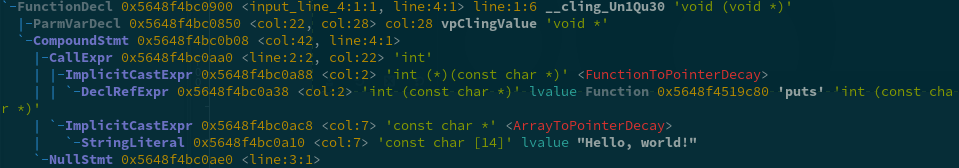
\includegraphics[width=\textwidth]{img/clang-ast-expl.png}
  };
  \draw<4->[expl line] (transform) -- ++(right:2in) node(transform_expl)[at end,anchor=west,black,solid]{%
    \ASTpre \sepRule $\rightarrow$ \sepRule \ASTpost
  };
  \draw<5->[expl line] (codegen) -- ++(right:2in) node(codegen_expl)[at end,anchor=west,expl]{%
    \resizebox{\textwidth}{!}{\usebox{\lstlistingCodeGen}}
  };
  \draw<6->[expl line] (callwrapper) -- ++(right:2in) node(callwrapper_expl)[at end,anchor=west,expl]{%
    [If $\exists$ top-level statement, get a pointer to the wrapper function and do indirect call]
  };

}


  \only<7->{
    \begin{tikzpicture}[remember picture,overlay]
      \node[anchor=east,opacity=.9] at ($(current page.east)+(-.85in,-.8in)$) {\tikz{
          \StickyNotePi[1.2in]{
            \begin{itemize}
            \item Deferred (implicit) template instantiations \textbf{must} be emitted; we do that by forcing a end-of-TU event!
            \item CodeGen: also involves linking (external symbol resolution, etc.)
            \end{itemize}
          }[3in]%
      }};
    \end{tikzpicture}
  }
\end{frame}

\begin{frame}[fragile]{Transactions}
  \begin{itemize}
    \itemsep=1ex

  \item AST is built incrementally

  \item \textbf{Transaction:} declarations that were parsed and emitted in a single step
    \begin{itemize}
    \item User-provided declarations
    \item Implicit template instatiations
    \item Deserialized declarations from a C++ module
    \end{itemize}

  \item And allows undoing it.  That's useful, e.g. after a failed parse
%    \begin{lstlisting}[style=c++]
%`\clingPrompt` auto p = std::make_unique<std::string>("Hi there!");
%`\clingPrompt` `\lsthl{p.size()}`
%  error: no member named 'size' in 'std::unique_ptr<std::basic_string<char>, std::default_delete<std::basic_string<char> > >'; did you mean to use '->' instead of '.'?
%  p.size()
%   ^
%    \end{lstlisting}
  \end{itemize}
\end{frame}

\begin{frame}[fragile]{Extensions}
  \begin{itemize}
    \itemsep=1ex

  \item Most extensions are implemented as an AST transformer
  \item Currently, there is support for
    \begin{itemize}
    \item \inlineCode{auto} synthesizing, e.g. \inlineCode{foobar = 42.0f;}
      \pause

    \item Protection against invalid pointer deferencing, e.g.
      \begin{lstlisting}[style=c++]
`\clingPrompt` *((int *)0xff00ff00) = 0;
Error in <HandleInterpreterException>: Trying to access a pointer that points to an invalid memory address.
Execution of your code was aborted.
ROOT_prompt_6:1:2: `\alert{warning:}` invalid memory pointer passed to a callee:
*((int *)0xff00ff00) = 0;
 ^~~~~~~~~~~~~~~~~~~
      \end{lstlisting}
      \pause

    \item Shadowing of definitions
      \begin{lstlisting}[style=c++]
`\clingPrompt` int foobar = 0;
`\clingPrompt` std::string foobar() { return "A string!"; }
      \end{lstlisting}
      \pause

    \item Printing / capturing the value of an expression
      \begin{lstlisting}[style=c++]
`\clingPrompt` foobar()
(std::string) "A string!"
      \end{lstlisting}
    \end{itemize}
  \end{itemize}
\end{frame}

\begin{frame}[fragile]{Debugging / Profiling of JIT'ed code}
  Cling also allows debugging JITed code and offers integration with Linux's \texttt{perf}, e.g.
  \vfill

  \begin{itemize}
  \item A breakpoint on interpreted code can be set and step-into after each statement

  \item It can generate a symbol file for \texttt{perf} -- Can be used together with Flamegraph%
    \footnote{Flamegraph: \url{\flamegraphURL}}!
  \end{itemize}
\end{frame}

\begin{frame}{The future of cling: \protect\texttt{clang-repl}}
  \begin{itemize}
    \itemsep=1ex

  \item Cling proved to perform okay in the context of the larger ROOT project at CERN

  \item Let's upstream the foundations of it back to the LLVM community so that
    \begin{itemize}
    \item The whole community can benefit from it
    \item Maintenance is easier in the long term
    \end{itemize}

  \item \texttt{clang-repl}: already in recent versions of LLVM --- \alert{Thanks, Vassil!}

  \item Slightly different to the design of cling, e.g. modeling of top-level statements is much more rubust
  \end{itemize}
\end{frame}
